\documentclass{bioinfo}
\copyrightyear{2013}
\pubyear{2013}

\begin{document}
\firstpage{1}

\title[libRoadRunner]{libRoadRunner: A High Performance SBML Compliant Simulator}
\author[Sample \textit{et~al}]{A. Somogyi\,$^{1,*}$, M. T. Karlsson\,$^{2}$, M. Swat\,$^{1}$ and H. M Sauro\,$^3$\footnote{to whom correspondence should be addressed}}
\address{$^{1,3}$Biocomplexity Institute, Indiana University, Simon Hall MSB1, 212 S. Hawthorne Drive, Bloomington, IN  47405-7003
\\
$^{2}$Dune Scientific, 10522 Lake City Way NE, \#302 Seattle WA \\
$^{3}$Department of Bioengineering, University of Washington, Seattle, WA, 98195}

\history{Version 0.75}

\editor{Associate Editor: XXXXX}

\maketitle

\begin{abstract}

\section{Summary:}
Here we describe libRoadRunner, a high performance SBML compliant simulator written in C/C++. Simulation speed is achieved by creating a LLVM backend of a model at runtime based on the loaded SBML. The primary motivation for developing libRoadRunner was to create a portable that would have superior performance to any other existing simulator, provide an extensible architecture, and a wide variety of functionality. In addition it would have superior support for event handling in addition to the normal features such as conservation analysis.

\section{Availability and Implementation:}
The core of libRoadRunner is written in C++ but with an additional thin layer that supports a pure C API. Users can link the library to other C++ applications or systems that can only link to C functions.  The library uses libSBML for SBML support, CVODE for differential equation implementation and event handling, NLEQ2 for solving nonlinear equations and LAPACK for stoichiometric analysis. The library is cross-platform and runs on Windows, Mac OS X and Linux. We also provide extensive bindings for Python. The library is open source and licensed under the Apache License, Version 2.0.

\section{Contact:} \href{hsauro@u.washington.edu}{hsauro@u.washington.edu}

\section{Supplementary information:}
Online documentation, build instructions and source code are available at http://www.libroadrunner.org

\end{abstract}

\section{Introduction}

There has been a long history~\citep{Bag01} of researchers developing biochemical network simulators. Most are monolithic making it very difficult to reuse the code for other applications. Recently there has been more interest in development reusable libraries. Most notable of these are COPASI, libSBMLSim, roadRunner, SOSLib and the Systems Biology Simulation Core Library (SBSCL). Each has strengths and weakness, for example COPASI has excellent support for optimization but its API can be challenging to use (see https://code.google.com/p/copasi-simple-api/), libSBMLSim passes all the tests in the SBML test suite but its API and functionality is somewhat limited, roadRunner is written in C\# which is excellent for .NET developers but less so for others, SOSLib is no longer supported but it has a reasonable API but does not support conservation analysis and finally SBSCL is written in Java which makes it an excellent choice for Java developers but less so for others and also doesn't support conservation analysis. All the libraries have performance issues and stability concerns (see benchmarking), most have problems tracking events except perhaps roadRunner and all have a non-extensible architectures.

Here we wish to describe libRoadRunner, a rewrite of the C\# roadRunner. libRoadRunner is written in C++ with an additional thin C API. The API is well structured with the modeler in mind and offers a wide range of functionality and specific methods for rapid access to the core to improve performance in realtime interactive environments. libRoadRunner supports a plugin extension mechanism making it possible to easily write extensions to the core (See Plugins). One of the key and novel features of libRoadRunner is that superior runtime performance is achieved through the use of LLVM (formerly Low Level Virtual Machine) which is designed for real-time optimization and dynamic compilation of application software. This has allowed us to develop the fastest biochemical simulator currently available. This is particularly important for large simulation applications such as ComuCell3D where 10,000 of cells are simulated simultaneously and performance is critical. Figure~\ref{fig:01} shows the architectural overview of libRoadRunner.

\begin{figure}[!htpb]%figure2
\centerline{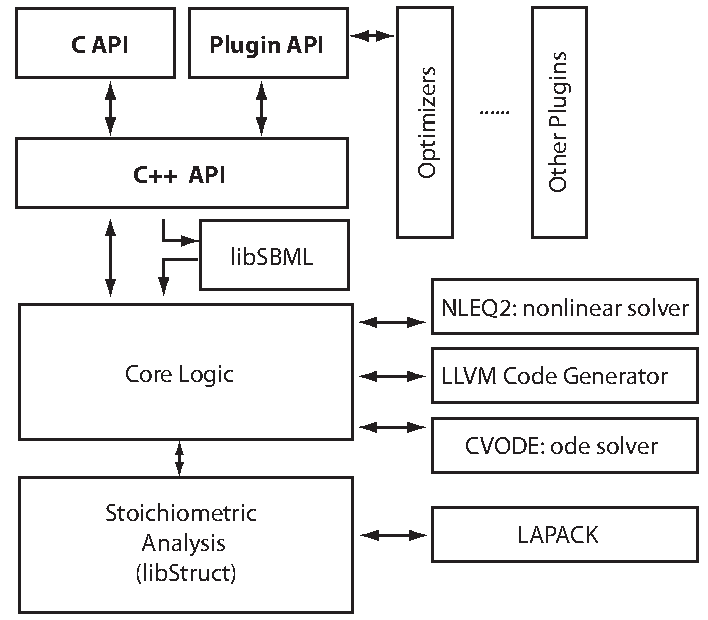
\includegraphics[scale=0.55]{roadRunnerOverview.pdf}}
\caption{Architectural Overview of libRoadRunner.}\label{fig:01}
\end{figure}

\begin{methods}
\section{Methods}

\subsection{Features}

List of features here

\subsection{LLVM Backend}

LLVM is a technology that allows dynamic compilation of code at runtime. This allows us to cast SBML models directly into native machine code at runtime. LLVM can generate runtime code for a large number of architectures, including on ARM (for example the  Raspberry Pi) but also for GPUs. In addition to GPU and CPU generated code the backend can be easily configured for other outputs. For example one option included with roadRunner is the ability to direct code generate to pure C code which can be useful for embedded systems where a C++ compiler is not available. Similarly simulation libraries can also be reconfigured such that a stochastic simulator would be incorporated. 

\subsection{Extensibility}

Extensibility was an importance consideration in the design of the roadRunner library as noted in the previous section. The easiest way to to add external new extensions by writing Python scripts, this is simple to do but with the disadvantage of potentially poorer performance. The alternative is to write native code plugins that can be loaded on demand by the roadRunner core. A plugin API is available as a pure C API so that plugins can be written in almost any language. Under Windows, a plugin is just a standard DLL. Plugins have full access to the roadRunner API which includes the ability to create new roadRunner instances. A primary advantage of plugins is that additional functionality can be developed without disturbing any of core roadRunner code. In addition, the plugin exposes a set of methods to allow generic access to any exported plugin functionality. This means that scripting languages such as Python can easily access a plugin without having to implement a new API for every plugin. Plugins also support a degree of runtime type information that allows graphical user interface applications to create user interfaces at runtime when the plugin is loaded. The roadRunner distribution comes with two plugins that illustrate how plugins can be built, these include a a plugin that implements the Levenberg-Marquardt algorithm (ref) that allows models to be fitted to experimental data and a smaller plugin that can be used to generate synthetic experimental data for testing the Levenberg-Marquardt plugin.


\subsection{Python API}

Two Python APIs were developed, a ctypes based library and customized SWIG binding. The SWIG binding is more comprehensive and Pythonic in its design and is the recommended interface to use on a daily basis. The ctypes Python interface is used to specifically test the C API. Here we briefly describe the SWIG bindings.

\subsection{Performance}

We compared three other simulator libraries with libRoadRunner (ref), these included libSBMLSim (ref), COPASI (ref) and Systems Biology Simulation Core Library (ref). We tested the ability pass the SBML test suite, the ability to simulate very large models and the ability to simulate systems with large numbers of events. Table~\ref{Tab:01} lists the times recorded from the four different libraries based on three different types of model. The first model is a moderate sized model that tests the general performance in integration and evaluating the differential equations. The second model tests the ability of the libraries to scale to very large models and the third library tests the ability of the library to deal with large number of discrete events. The timings also include the amount of time requite to load the SBML model and compile it to executable code.
%
\begin{table}[!t]
\processtable{All times are in milliseconds. Test models are available at libroadrunner.org\label{Tab:01}}
{\begin{tabular}{llll}\toprule
Application & Simulation & Large Models & Event Handling\\\midrule
libRoadRunner & 23 & 45 & 67  \\
COPASI & 200 & 400 & fail\\
libSBMLSim & 450 & fail & fail\\
SBSCL & 500 & 800 & fail \\ \botrule
\end{tabular}}{}
\end{table}

\subsection*{Implementation Details}

The dedicated web site, libroadrunner.org includes all the necessary information concerning libRoadRunner including documentation for the C++ and C API, and documentation for the Python SWIG binding. Full build instructions are provided for Windows and Mac OS X. Build instructions for specific Linux disruptions can be obtained upon request particularly XYZ and ABC. All source code is stored on Github, documentation is generated via Doxygen and sphinc for Python. The build system is based around CMake, Linux binaries are generated using GCC, Mac binaries via CLang \citealp{Boffelli03} and Windows binaries via Visual Studio 2010. Binaries are provided for Windows, Mac OS X, including binaries for Python 2.7 on Windows and Mac OS X.

\end{methods}

\section{Discussion}

In this application note we describe a new high performance SBML compliant simulator. The reason for developing libRoadRunner was to satisfy a number of specific applications that require high performance, good SBML compatibility and broad functionality. These applications include interactive desktop simulation, multicellular simulations requiring 10,000 of simultaneous simulations, and multi-session needs for web based interactive simulation.  For the future we are planning a number of additional features, these include new plugins, particularly alternative optimizers, and a bifurcation analysis plugin. Expand this: Currently used by: CompuCell3D, JDesigner, Tellurium, sysb.io

\section*{Acknowledgement}
We wish to acknowledge Frank Bergmann who together with Herbert Sauro wrote the original roadRunner library in C\#. In addition libStruct, the structural analysis library previously developed by Frank Bergmann and Ravi Rao. We wish to also thank Michal Galdzicki who assisted in putting together the libroadrunner.org website. Finally we wish to thank Stanley Gu for testing libRoadRunner in his web based environment.

\paragraph{Funding\textcolon} Work supported by the National Institute of General Medical Sciences of the National Institutes of Health under award numbers R01-GM081070. The content is solely the responsibility of the authors and does not necessarily represent the official views of the National Institutes of Health.

%\bibliographystyle{natbib}
%\bibliographystyle{achemnat}
%\bibliographystyle{plainnat}
%\bibliographystyle{abbrv}
%\bibliographystyle{bioinformatics}
%
%\bibliographystyle{plain}
%
%\bibliography{Document}


\begin{thebibliography}{}
\bibitem[Bofelli {\it et~al}., 2000]{Boffelli03} Bofelli,F., Name2, Name3 (2003) Article title, {\it Journal Name}, {\bf 199}, 133-154.

\bibitem[Bag {\it et~al}., 2001]{Bag01} Bag,M., Name2, Name3 (2001) Article title, {\it Journal Name}, {\bf 99}, 33-54.

\bibitem[Yoo \textit{et~al}., 2003]{Yoo03}
Yoo,M.S. \textit{et~al}. (2003) Oxidative stress regulated genes
in nigral dopaminergic neurnol cell: correlation with the known
pathology in Parkinson's disease. \textit{Brain Res. Mol. Brain
Res.}, \textbf{110}(Suppl. 1), 76--84.

\bibitem[Lehmann, 1986]{Leh86}
Lehmann,E.L. (1986) Chapter title. \textit{Book Title}. Vol.~1, 2nd edn. Springer-Verlag, New York.

\bibitem[Crenshaw and Jones, 2003]{Cre03}
Crenshaw, B.,III, and Jones, W.B.,Jr (2003) The future of clinical
cancer management: one tumor, one chip. \textit{Bioinformatics},
doi:10.1093/bioinformatics/btn000.

\bibitem[Auhtor \textit{et~al}. (2000)]{Aut00}
Auhtor,A.B. \textit{et~al}. (2000) Chapter title. In Smith, A.C.
(ed.), \textit{Book Title}, 2nd edn. Publisher, Location, Vol. 1, pp.
???--???.

\bibitem[Bardet, 1920]{Bar20}
Bardet, G. (1920) Sur un syndrome d'obesite infantile avec
polydactylie et retinite pigmentaire (contribution a l'etude des
formes cliniques de l'obesite hypophysaire). PhD Thesis, name of
institution, Paris, France.

\end{thebibliography}
\end{document}
